%!TEX root = ../thesis.tex

\chapter{Experimentelle Evaluation}
\label{chap:evaluation}
In diesem Kapitel wird die Zuverlässigkeit und Präzision der Implementierung analysiert. Zu diesem Zweck wird die Erkennungsquote in verschiedenen Aspekten betrachtet.

Dabei wurden die Daten auf einem System mit Ubuntu 16.04 LTS und OpenCV Version 3.1 für Python 3 erfasst. Die hierbei genutzte Hardware ist ein Intel i7 4790k, mit 4 GHz und vier physischen Kernen. Zudem wurde eine Nvidia GTX 970 mit CUDA Support genutzt.
Die eingesetzte Kamera ist eine Logitech C310, welche über eine HD Auflösung mit  $1.280\times720$ bei $30FPS$ verfügt. 

\begin{figure}[ht]
\centering
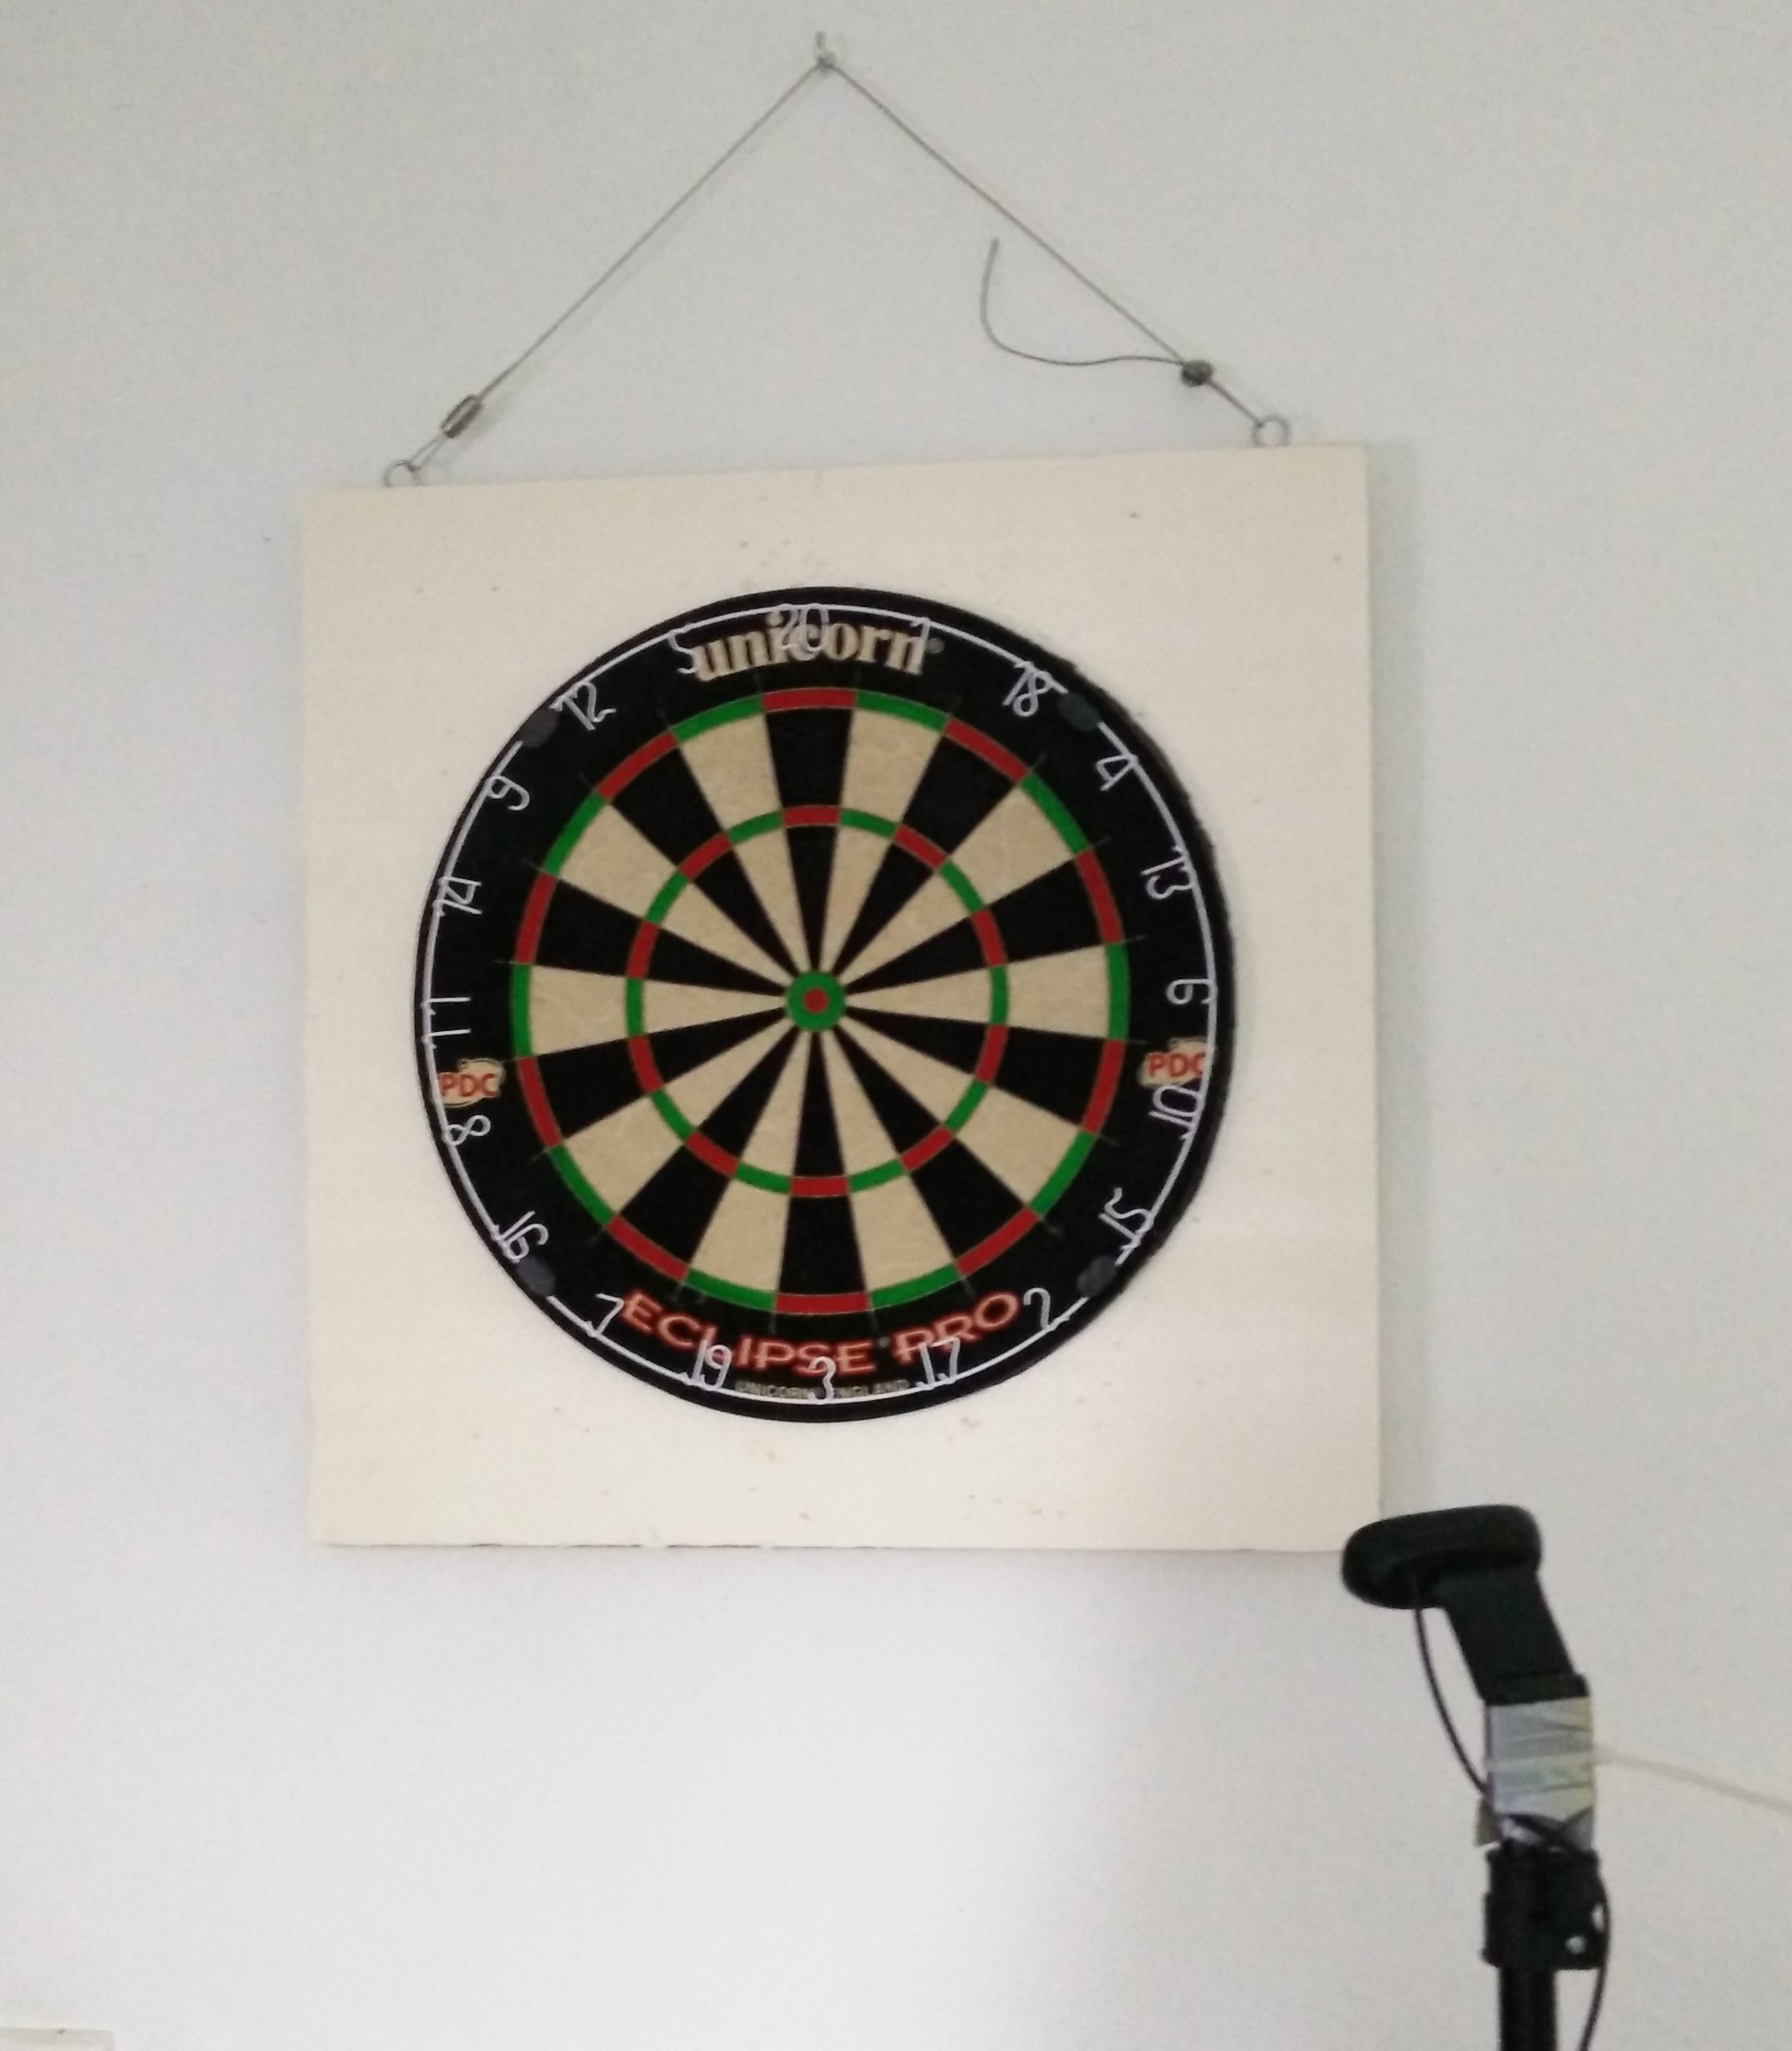
\includegraphics[width=0.6\textwidth]{media/testsetup}\\
\caption{\textbf{Zur Evaluation genutztes Setup}}
\label{Fig:testsetup}
\end{figure}
In Abbildung \prettyref{Fig:testsetup} ist das Setup abgebildet. Dabei wurde die Kamera so aufgestellt, dass sie seitlich von unten auf das Dartboard gerichtet ist. Damit wird verhindert, dass die Kamera sich in der Flugbahn der Darts befindet. Zudem wurden konstante Lichtverhältnisse geschaffen, indem die Dartbescheibe passiv mit zwei Studiolampen ausgeleuchtet wurde.
\begin{figure}[ht]
\centering
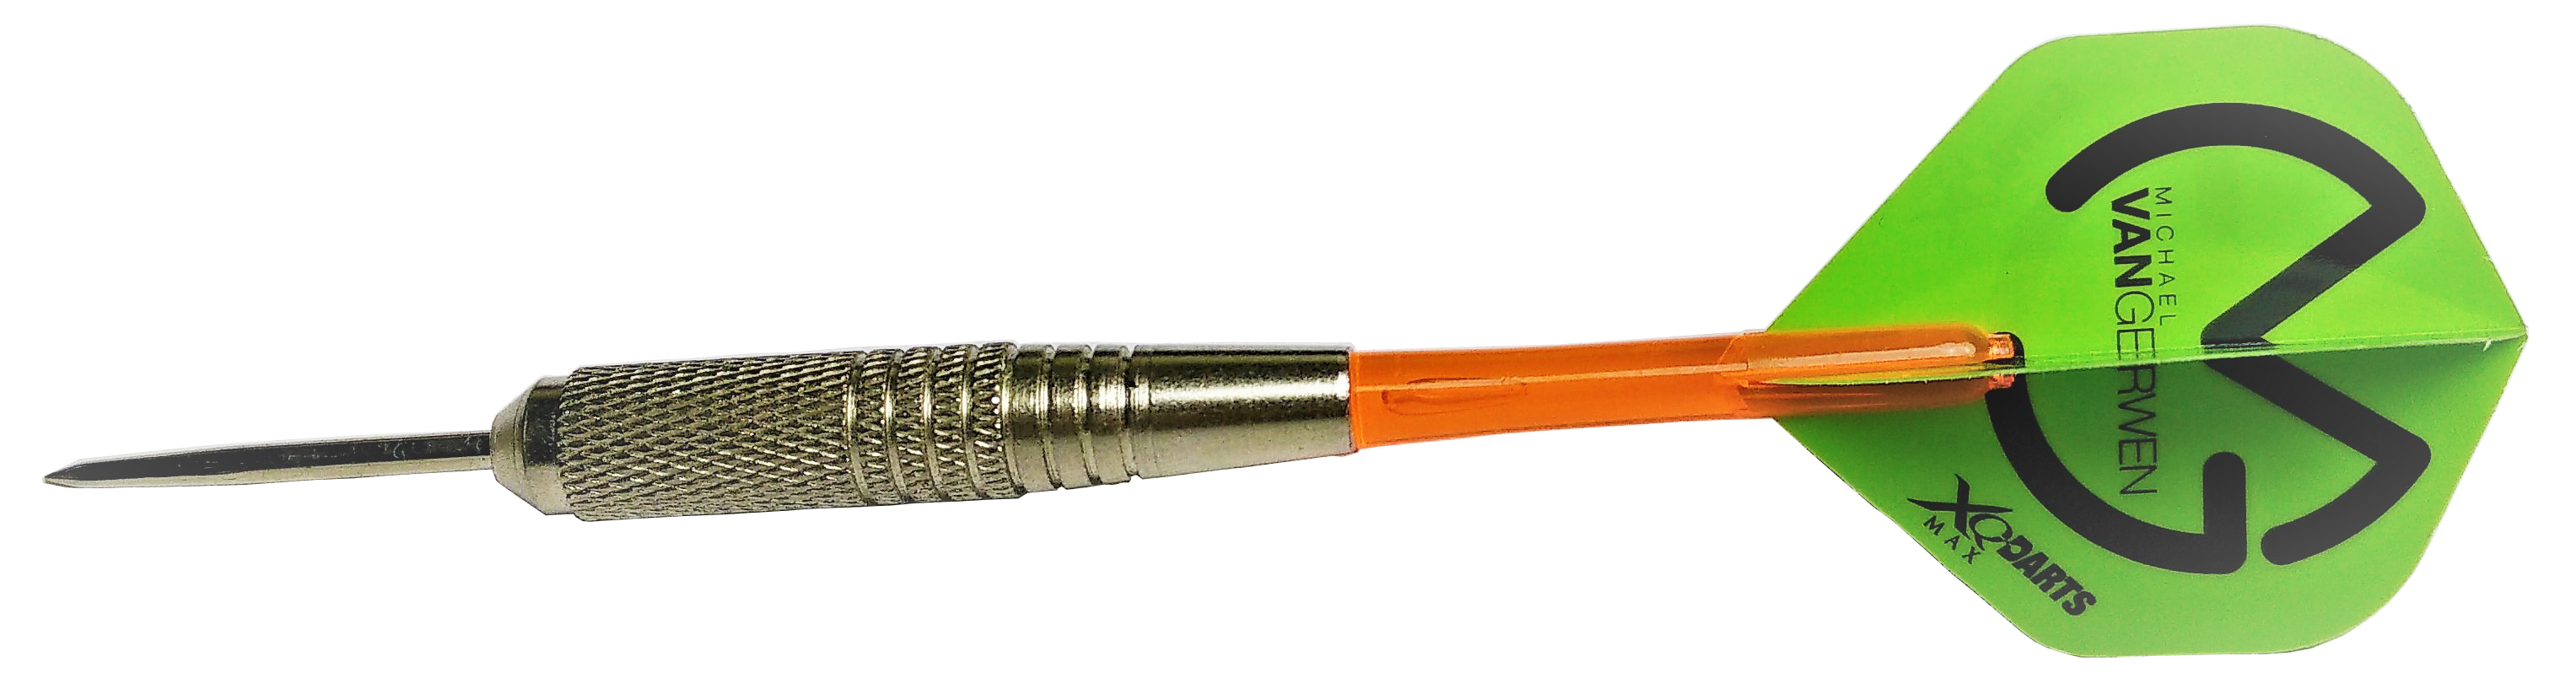
\includegraphics[width=\textwidth]{media/MyDart.png}\\
\caption{\textbf{Zur Evaluation genutzte Darts}}
\label{Fig:mydart}
\end{figure}

Zur Erfassung wurden rund 1000  Testwürfe durchgeführt und aufgezeichnet. Damit eine möglichst große Streuung der Würfe gegeben ist, wurde nicht im klassischen Turniermodus vorgegangen. Stattdessen wurde, der im \prettyref{sec:motivation} genannte, Modus "`Rennen"' genutzt, da es bei diesem das Ziel ist, jedes Feld auf dem Dartboard zu treffen. Würden die Würfe im Turniermodus gesammelt, so hätten sich die Würfe stark auf eine Region konzentriert.


\section*{Ergebnisse}
\label{sec:results}
Zunächst wurden alle Daten betrachtet und die fünf Spitzen dem real erzielten Feld gegenübergestellt. Zum einen wurde der prozentuale Anteil der korrekt ermittelten Felder bestimmt, um eine Übersicht zu vermitteln, welche der verschiedenen Varianten der Spitzen-Erkennung die erfolgreichste ist. Zum anderen wurde bei den nicht korrekt erkannten Darts betrachtet wie groß die Abweichung zum tatsächlichen Ausgang ist. Hierfür wurde überprüft, ob sich das erkannte Feld in der direkten Nachbarschaft zum real erzielten Feld befindet. So wurden die Fehlerkennungen aufgeschlüsselt und in "`grundlegend falsch"' sowie "`als direkter Nachbar"' erkannt.


In Abbildung \prettyref{Fig:plainchart}  sind alle Daten unbereinigt gegenübersgestellt. Zu erkennen ist, dass eine reine Erkennungsrate von rund $87\%$ (grün markiert) erzielt wurde. In Tabelle \prettyref{Tab:plaindata} sind die Daten abzulesen. Dabei zeigt sich, dass die erste Variante der Bestimmung der Dart-Spitze die zuverlässigste ist. Von den rund $12\%$ der nicht korrekt erkannten Darts liegt ein großteil in der direkten Nachbarschaft des real erzielten Feldes (gelb markiert). Tieferliegende Schwierigkeiten bei der Erkennung unterlagen somit nur rund $2\%$ der Würfe.
\begin{figure}[ht]
\centering
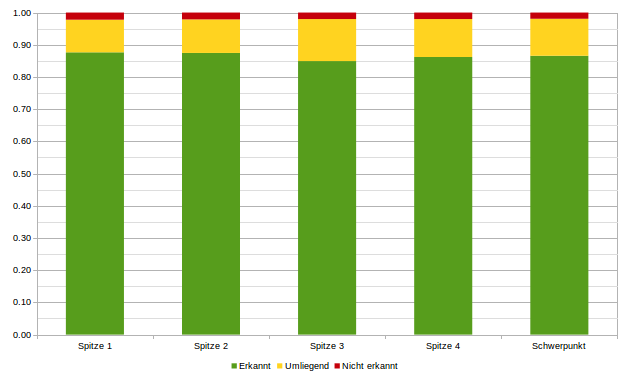
\includegraphics[width=\textwidth]{media/chartplain}\\
\caption{\textbf{Erkannte Spitzen in Gegenüberstelltung}}
\label{Fig:plainchart}
\end{figure}

\begin{table}[htbp]
\caption{Daten der erkannten Spitzen in Gegenüberstelltung}
\begin{tabular}{|l|r|r|r|r|r|}
\hline
 & \multicolumn{1}{l|}{Spitze 1} & \multicolumn{1}{l|}{Spitze 2} & \multicolumn{1}{l|}{Spitze 3} & \multicolumn{1}{l|}{Spitze 4} & \multicolumn{1}{l|}{Schwerpunkt} \\ \hline
Erkannt & 87.64\% & 87.46\% & 84.94\% & 86.20\% & 86.58\% \\ \hline
Umliegend & 10.14\% & 10.42\% & 13.03\% & 11.78\% & 11.49\% \\ \hline
Nicht erkannt & 2.22\% & 2.12\% & 2.03\% & 2.02\% & 1.93\% \\ \hline
\end{tabular}
\label{Tab:plaindata}
\end{table}

Ebenso wurde ein weiterer wichtiger Aspekt betrachtet. Aufgrund des, einzelnen und unbeweglichen, Standpunktes der Kamera kann es zu einer Verdeckung der Darts kommen. So kann es vorkommen, dass Darts partiell, oder gänzlich, verdeckt werden. Bei der Aufzeichnung der Testdaten wurde, zusätzlich zu der Information über das real erzielte Feld, gespeichert, ob eine Verdeckung auftrat. Dies war bei $5.5\%$ der Testwürfe der Fall.
Die in Abbildung \prettyref{Fig:chartcovert} gegenübergestellten Daten wurden nach Verdeckung gefiltert. So wird dargestellt, wie sich Verdeckung auf die Erkennungsrate auswirkt. Es ist zu erkennen, dass nur $37$ bis $45\%$ erfolgreich erkannt werden konnte und in etwa der gleiche Anteil in der direkten Nachbarschaft identifiziert wurde. 
Ersichtlich ist, dass die Verdeckung der Darts eines der größeren Probleme darstellt.

\begin{figure}[ht]
\centering
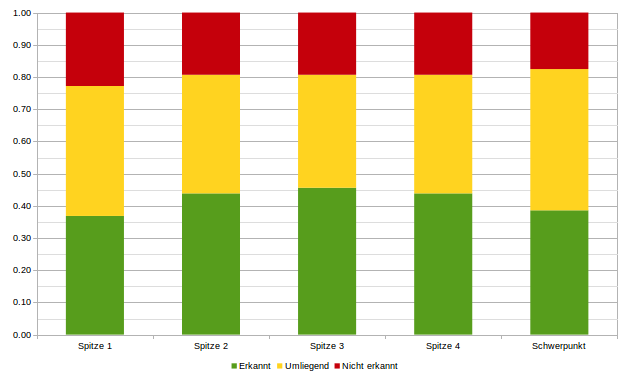
\includegraphics[width=\textwidth]{media/chartonlycovert}\\
\caption{\textbf{Erkannte Spitzen der verdeckten Darts in Gegenüberstellung}}
\label{Fig:chartcovert}
\end{figure}

\begin{table}[htbp]
\caption{Daten der erkannten Spitzen verdeckter Darts in Gegenüberstellung}
\begin{tabular}{|l|r|r|r|r|r|}
\hline
 & \multicolumn{1}{l|}{Spitze 1} & \multicolumn{1}{l|}{Spitze 2} & \multicolumn{1}{l|}{Spitze 3} & \multicolumn{1}{l|}{Spitze 4} & \multicolumn{1}{l|}{Schwerpunkt} \\ \hline
Erkannt & 36.84\% & 43.86\% & 45.61\% & 43.86\% & 38.60\% \\ \hline
Umliegend & 40.35\% & 36.84\% & 35.09\% & 36.84\% & 43.86\% \\ \hline
Nicht erkannt & 22.81\% & 19.30\% & 19.30\% & 19.30\% & 17.54\% \\ \hline
\end{tabular}
\label{}
\end{table}


Als letztes wurde die Erkennungsrate einzelner Darts betrachtet. Zu diesem Zweck wurden die Daten nach unverdeckten Darts gefiltert, was in Abbildung \prettyref{Fig:chartuncovert} dargestellt ist. So steigt die Erkennungsrate auf circa $90\%$. Damit würde nur $1\%$ der Darts zu einer kompletten Fehlerkennung führen. 

\begin{figure}[ht]
\centering
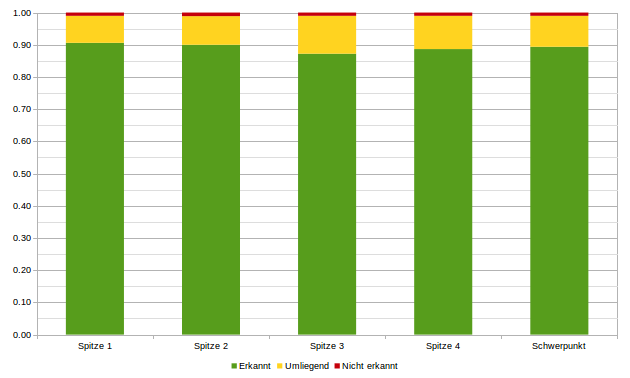
\includegraphics[width=\textwidth]{media/chartwithoutcovert}\\
\caption{\textbf{Erkannte Spitzen der unverdeckten Darts in Gegenüberstellung}}
\label{Fig:chartuncovert}
\end{figure}

\begin{table}[ht]
\caption{Daten der erkannten Spitzen der unverdeckten Darts in Gegenüberstellung}
\begin{tabular}{|l|r|r|r|r|r|}
\hline
 & \multicolumn{1}{l|}{Spitze 1} & \multicolumn{1}{l|}{Spitze 2} & \multicolumn{1}{l|}{Spitze 3} & \multicolumn{1}{l|}{Spitze 4} & \multicolumn{1}{l|}{Schwerpunkt} \\ \hline
Erkannt & 90.60\% & 89.99\% & 87.23\% & 88.66\% & 89.38\% \\ \hline
Umliegend & 8.38\% & 8.89\% & 11.75\% & 10.32\% & 9.60\% \\ \hline
Nicht erkannt & 1.02\% & 1.12\% & 1.02\% & 1.02\% & 1.02\% \\ \hline
\end{tabular}
\label{}
\end{table}


Über alle Betrachtungen ist zu sagen, dass insgesamt die erste Variante der Spitzen-Erkennung die stabilste ist. Zudem ist zu erkennen, dass es zwei größere Probleme in der Implementierung gibt. Zum einen verursacht die Verdeckung hohe Fehlerkennung und zum anderen tritt eine leichte Ungenauigkeit auf, sodass die Erkennung eines der benachbarten Felder auftritt.


